\documentclass[cjk]{beamer}
\usepackage{CJK}						%windows
\usepackage{ccmap}
\usepackage{float}
%\usepackage{CJKutf8}					%Linux
%\usepackage{CJKulem}
\usepackage{courier}
\usepackage{makeidx}
\usepackage{amssymb}
\usepackage{amsmath}
\usepackage{amsfonts}
\usepackage{fancyhdr}
\usepackage{lastpage}
\usepackage{graphicx}
\usepackage{latexsym}
\usepackage{multicol}
\usepackage{multirow}
\usepackage[linesnumbered,ruled,longend]{algorithm2e}
\usepackage{extramarks}
\usepackage{indentfirst}
\usepackage{hyperref}
\usepackage{listings}

\newcommand{\song}{\CJKfamily{song}} % ����
\newcommand{\hei}{\CJKfamily{hei}}   % ����
\newcommand{\fs}{\CJKfamily{fs}}	 % ����
\newcommand{\kai}{\CJKfamily{kai}}   % ����
\newcommand{\li}{\CJKfamily{li}}     % ����
\newcommand{\you}{\CJKfamily{you}} 	 % ��Բ

\usetheme{Boxes}
\useinnertheme{rectangles}
\useoutertheme{miniframes}

\title{Some Math Notes}
\author{Yuchong Pan}

\begin{document}

\begin{CJK}{GBK}{kai}

	\SetKwBlock{Function}{Function}{end}

	\title{Some Math Notes}
	\author{Yuchong Pan}
	\institute{Faculty of Science, University of British Columbia}
	\date{\today}
	\maketitle

    \section{}
    \begin{frame}
        \centering
        \huge Happy Birthday to \color{orange}{liyang21} \color{black}{!}
    \end{frame}

	\begin{frame}%[shrink]
		\frametitle{Outline}
		%\begin{multicols}{2}
			\tableofcontents
		%\end{multicols}
	\end{frame}

    \section{Linear Algebra}
    \begin{frame}%[shrink]
		\frametitle{Outline}
		%\begin{multicols}{2}
			\tableofcontents[currentsection,currentsubsection]
		%\end{multicols}
	\end{frame}

    \subsection{Gaussian Elimination}
    \begin{frame}{Matrix and System of Equations}
        \begin{itemize}
            \pause \item A \textbf{system of linear equations} consisting of $m$ equations and of $n$ unknown variables is given as
                \begin{equation}
                    \nonumber
                    \begin{cases}
                        a_{11}x_1 + a_{12}x_2 + \cdots + a_{1n}x_n = b_1 \\
                        a_{21}x_1 + a_{22}x_2 + \cdots + a_{2n}x_n = b_2 \\
                        \quad \cdots \\
                        a_{m1}x_1 + a_{m2}x_2 + \cdots + a_{mn}x_n = b_m
                    \end{cases}
                \end{equation}
        \end{itemize}
    \end{frame}
    \begin{frame}{Matrix and System of Equations}
        \begin{itemize}
            \pause \item The system of equations above can be written as an augmented matrix
                \begin{equation}
                    \nonumber
                    \left(
                    \begin{array}{cccc|c}
                        a_{11} & a_{12} & \cdots & a_{1n} & b_1 \\
                        a_{21} & a_{22} & \cdots & a_{2n} & b_2 \\
                        \vdots & & & & \vdots \\
                        a_{m1} & a_{m2} & \cdots & a_{mn} & b_m
                    \end{array}
                    \right)
                \end{equation}
        \end{itemize}
    \end{frame}
    \begin{frame}{Row Operations}
        \begin{itemize}
            \pause \item There are 3 types of elementary row operations:
            \pause \item \textbf{Type 1}: Swap the positions of two rows.
            \pause \item \textbf{Type 2}: Multiply a row by a nonzero scalar.
            \pause \item \textbf{Type 3}: Add to one row a scalar multiple of another.
            \pause \item If a matrix is associated to a system of linear equations, then these three types of row operations do not change the solution set.
        \end{itemize}
    \end{frame}
    \begin{frame}{Row Echelon Form}
        \begin{itemize}
            \pause \item For each row in a matrix, if the row does not consist of only zeros, then the left-most nonzero entry in called the \textbf{leading coefficient} (or \textbf{pivot}) of that row.
            \pause \item A matrix is in the \textbf{row echelon form} if
                \begin{itemize}
                    \item all nonzero rows are above any rows of all zeros, and
                    \item the leading coefficient of a nonzero row is always strictly to the right of the leading coefficient of the row above it.
                \end{itemize}
            \pause \item Hence, the lower left part of the matrix contains only zeros.
            \pause \item For example, the following matrix is in the row echelon form, and its leading coefficients are shown in red.
                \begin{equation}
                    \nonumber
                    \left(
                    \begin{matrix}
                        0 & \color{red}{2} & 1 & -1 \\
                        0 & 0 & \color{red}{3} & 1 \\
                        0 & 0 & 0 & 0
                    \end{matrix}
                    \right)
                \end{equation}
        \end{itemize}
    \end{frame}
    \begin{frame}{Gaussian Elimination}
        \begin{itemize}
            \pause \item The procedure of using the 3 types of the elementary row operations to transform an augmented matrix associated to a system of linear equations to the row echelon form is called \textbf{Gaussian elimination} (or \textbf{forward elimination}).
            \pause \item If two leading coefficients are in the same column, then a row operation of type 3 could be used to make one of those coefficients zero.
            \pause \item Then, by using the row operations of type 1 (i.e., the row swapping operations), one can always order the rows so that, for every nonzero rows, the leading coefficient is to the right of the leading coefficient of the row above.
        \end{itemize}
    \end{frame}
    \begin{frame}{Example}
        \begin{itemize}
            \pause \item The original augmented matrix is
                \begin{equation}
                    \nonumber
                    \left(
                    \begin{array}{ccc|c}
                        2 & 1 & -1 & 8 \\
                        -3 & -1 & 2 & -11 \\
                        -2 & 1 & 2 & -3
                    \end{array}
                    \right)
                \end{equation}
            \pause \item After the row operations $L_2 + \frac{3}{2} L_1 \rightarrow L_2$ and $L_3 + L_1 \rightarrow L_3$, the augmented matrix is transformed to
                \begin{equation}
                    \nonumber
                    \left(
                    \begin{array}{ccc|c}
                        2 & 1 & -1 & 8 \\
                        0 & \frac{1}{2} & \frac{1}{2} & 1 \\
                        0 & 2 & 1 & 5
                    \end{array}
                    \right)
                \end{equation}
        \end{itemize}
    \end{frame}
    \begin{frame}{Example}
        \begin{itemize}
            \pause \item Then, after the row operation $L_3 - 4L_2 \rightarrow L_3$, the augmented matrix is transformed to
                \begin{equation}
                    \nonumber
                    \left(
                    \begin{array}{ccc|c}
                        2 & 1 & -1 & 8 \\
                        0 & \frac{1}{2} & \frac{1}{2} & 1 \\
                        0 & 0 & -1 & 1
                    \end{array}
                    \right)
                \end{equation}
            \pause \item The matrix is now in the row echelon form (or the triangular form).
        \end{itemize}
    \end{frame}
    \begin{frame}{Number of Solutions}
        \begin{itemize}
            \pause \item If the row echelon form has a row in the following form:
                \begin{equation}
                    \nonumber
                    \left(
                    \begin{array}{cccc|c}
                        0 & 0 & \cdots & 0 & a
                    \end{array}
                    \right)
                \end{equation}
                where $a \neq 0$, then this system of linear equations is \textbf{inconsistent}, i.e., has no solutions.
        \end{itemize}
    \end{frame}
    \begin{frame}{Number of Solutions}
        \begin{itemize}
            \pause \item If the number of variables equals the number of nonzero rows in the row echelon form, then the system of linear equations has a unique solution.
            \pause \item Otherwise, if the number of nonzero rows in the row echelon form is greater than the number of variables, then the system of linear equations has infinitely many solutions.
            \pause \item If the $k$-th column has no leading coefficients, then the variable $x_k$ is said to be a \textbf{free variable}, meaning that $x_k$ can be any real number.
            \pause \item Hence, for each given tuple of free variables, the system of linear equations has exactly one solution.
        \end{itemize}
    \end{frame}
    \begin{frame}{Example}
        \begin{itemize}
            \pause \item For example, the matrix
                \begin{equation}
                    \nonumber
                    \left(
                    \begin{array}{ccccc|c}
                        1 & 1 & 1 & 1 & 1 & 1 \\
                        0 & 0 & 1 & 1 & 2 & 0 \\
                        0 & 0 & 0 & 0 & 1 & 3 \\
                        0 & 0 & 0 & 0 & 0 & 0 \\
                        0 & 0 & 0 & 0 & 0 & 0
                    \end{array}
                    \right)
                \end{equation}
                has infinitely many solutions and 2 variables $x_2$ and $x_4$.
        \end{itemize}
    \end{frame}
    \begin{frame}{Example}
        \begin{itemize}
            \pause \item Given that $x_2 = x_4 = 0$, then $x_5 = 3, x_3 = -6, x_1 = 4$, and hence
                \begin{equation}
                    \nonumber
                    \begin{cases}
                        x_1 = 4 \\
                        x_2 = 0 \\
                        x_3 = -6 \\
                        x_4 = 0 \\
                        x_5 = 3
                    \end{cases}
                \end{equation}
                is a solution to the system of equations.
        \end{itemize}
    \end{frame}
    \begin{frame}{Reduced Row Echelon Form}
        \begin{itemize}
            \pause \item A matrix is said to be in the \textbf{reduced row echelon form} if
                \begin{itemize}
                    \item it is in the row echelon form,
                    \item all of the leading coefficients are equal to 1, and
                    \item in every column containing a leading coefficient, all of the other entries in that column are zero.
                \end{itemize}
            \pause \item The second condition can be achieved by the elementary row operations of type 2, and the third condition can be achieved by the elementary row operations of type 3.
            \pause \item This procedure is called \textbf{Gauss-Jordan elimination} (or the \textbf{back substitution}).
            \pause \item The total time complexity of forward elimination and back substitution is $O(n ^ 3)$.
        \end{itemize}
    \end{frame}
    \begin{frame}{Example}
        \begin{itemize}
            \pause \item Assuming that a matrix has been transformed to the row echelon form as follows.
                \begin{equation}
                    \nonumber
                    \left(
                    \begin{array}{ccc|c}
                        2 & 1 & -1 & 8 \\
                        0 & \frac{1}{2} & \frac{1}{2} & 1 \\
                        0 & 0 & -1 & 1
                    \end{array}
                    \right)
                \end{equation}
            \pause \item After 2 row operations $L_2 + \frac{1}{2} L_3 \rightarrow L_2$ and $L_1 - L_3 \rightarrow L_1$, then the matrix is transformed to
                \begin{equation}
                    \nonumber
                    \left(
                    \begin{array}{ccc|c}
                        2 & 1 & 0 & 7 \\
                        0 & \frac{1}{2} & 0 & \frac{3}{2} \\
                        0 & 0 & -1 & 1
                    \end{array}
                    \right)
                \end{equation}
        \end{itemize}
    \end{frame}
    \begin{frame}{Example}
        \begin{itemize}
            \pause \item Then, after another 2 row operations $2L_2 \rightarrow L_2$ and $-L_3 \rightarrow L_3$, we have
                \begin{equation}
                    \nonumber
                    \left(
                    \begin{array}{ccc|c}
                        2 & 1 & 0 & 7 \\
                        0 & 1 & 0 & 3 \\
                        0 & 0 & 1 & -1
                    \end{array}
                    \right)
                \end{equation}
            \pause \item Finally, after $L_1 - L_2 \rightarrow L_1$ and $\frac{1}{2} L_1 \rightarrow L_1$, the matrix is transformed to
                \begin{equation}
                    \nonumber
                    \left(
                    \begin{array}{ccc|c}
                        1 & 0 & 0 & 2 \\
                        0 & 1 & 0 & 3 \\
                        0 & 0 & 1 & -1
                    \end{array}
                    \right)
                \end{equation}
        \end{itemize}
    \end{frame}
    \begin{frame}{Example}
        \begin{itemize}
            \pause \item The matrix is now in the reduced row echelon form, and we obtain the unique solution to the system of linear equations:
                \begin{equation}
                    \nonumber
                    \begin{cases}
                        x_1 = 2 \\
                        x_2 = 3 \\
                        x_3 = -1
                    \end{cases}
                \end{equation}
        \end{itemize}
    \end{frame}
    \begin{frame}{System of XOR Equations}
        \begin{itemize}
            \pause \item A \textbf{system of XOR equations}
                \begin{equation}
                    \nonumber
                    \begin{cases}
                        a_{11}x_1 \otimes a_{12}x_2 \otimes \cdots \otimes a_{1n}x_n = b_1 \\
                        a_{21}x_1 \otimes a_{22}x_2 \otimes \cdots \otimes a_{2n}x_n = b_2 \\
                        \quad \cdots \\
                        a_{m1}x_1 \otimes a_{m2}x_2 \otimes \cdots \otimes a_{mn}x_n = b_m
                    \end{cases}
                \end{equation}
                where $a_{ij}, b_i, x_j \in \{0, 1\}$ and $\otimes$ is the XOR operation, can be also written as an augmented matrix
                \begin{equation}
                    \nonumber
                    \left(
                    \begin{array}{cccc|c}
                        a_{11} & a_{12} & \cdots & a_{1n} & b_1 \\
                        a_{21} & a_{22} & \cdots & a_{2n} & b_2 \\
                        \vdots & & & & \vdots \\
                        a_{m1} & a_{m2} & \cdots & a_{mn} & b_m
                    \end{array}
                    \right)
                \end{equation}
        \end{itemize}
    \end{frame}
    \begin{frame}{System of XOR equations}
        \begin{itemize}
            \pause \item Since the XOR operation can be regarded as the addition operation on the residue system modulo 2, then the 3 types of the elementary row operations are compatible with sytems of XOR equations.
            \pause \item Hence, Gaussian elimination can be applied to solve systems of XOR equations.
            \pause \item Note that there might be many free variables in a system of XOR equations.
            \pause \item Furthermore, we can use the bitset to optimize Gaussian elimination, and hence a system of XOR equations can be solved in time $O\left(\frac{n ^ 3}{w}\right)$.
        \end{itemize}
    \end{frame}

    \subsection{Determinant}
    \begin{frame}{$2 \times 2$ Matrices}
        \begin{itemize}
            \pause \item The determinant of a $2 \times 2$ matrix is defined by
                \begin{equation}
                    \nonumber
                    \left|
                    \begin{array}{cc}
                        a & b \\
                        c & d
                    \end{array}
                    \right| = ad - bc
                \end{equation}
            \pause \item The absolute value of $ad - bc$ is the area of the parallelogram with vertices at $(0, 0)$, $(a, b)$, $(a + c, b + d)$, and $(c, d)$.
                \begin{figure}
                  \centering
                  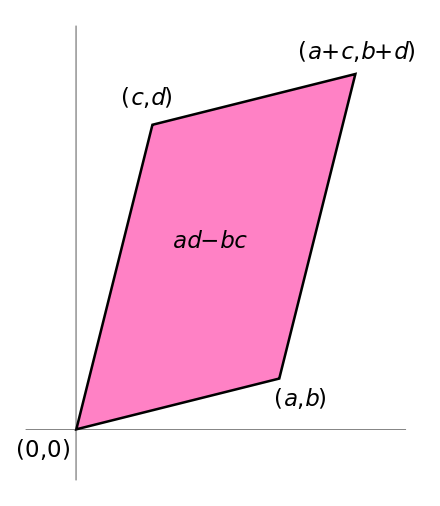
\includegraphics[width=1in]{440px-Area_parallellogram_as_determinant.png}
                \end{figure}
        \end{itemize}
    \end{frame}
    \begin{frame}{$2 \times 2$ Matrices}
        \begin{itemize}
            \pause \item Suppose $\vec{a} = (a, b)$ and $\vec{b} = (c, d)$ are two vectors defining the parallelogram.
            \pause \item Then $ad - bc$ is the \textbf{oriented area} of the parallelogram, which is negative when the angle from the first to the second vector defining the parallelogram turns in a clockwise direction, and positive otherwise.
            \pause \item The \textbf{signed area} can be expressed as $$Signed~Area = |\vec{a}| |\vec{b}| \sin \theta$$
        \end{itemize}
    \end{frame}
    \begin{frame}{$2 \times 2$ Matrices}
        \begin{itemize}
            \pause \item Suppose $\theta ' = \frac{\pi}{2} - \theta$ is the complementary angle to $\theta$, and $\vec{a} ^ \bot = (-b, a)$ is the perpendicular vector to $\vec{a}$.
            \pause \item Hence,
                \begin{equation}
                    \nonumber
                    \begin{aligned}
                        Signed~Area &= |\vec{a}| |\vec{b}| \sin \theta = |\vec{a} ^ \bot| |\vec{b}| \cos \theta ' \\
                        &=
                        \left(
                        \begin{matrix}
                            -b \\
                            a
                        \end{matrix}
                        \right)
                        \cdot
                        \left(
                        \begin{matrix}
                            c \\
                            d
                        \end{matrix}
                        \right)
                        = ad - bc
                    \end{aligned}
                \end{equation}
        \end{itemize}
    \end{frame}
    \begin{frame}{$3 \times 3$ Matrices}
        \begin{itemize}
            \pause \item The determinant of a $3 \times 3$ matrix is defined by
                \begin{equation}
                    \nonumber
                    \begin{aligned}
                        \left|
                        \begin{matrix}
                            a & b & c \\
                            d & e & f \\
                            g & h & i
                        \end{matrix}
                        \right|
                        &= a
                        \left|
                        \begin{matrix}
                            e & f \\
                            h & i
                        \end{matrix}
                        \right|
                        - b
                        \left|
                        \begin{matrix}
                            d & f \\
                            g & i
                        \end{matrix}
                        \right|
                        + c
                        \left|
                        \begin{matrix}
                            d & e \\
                            g & h
                        \end{matrix}
                        \right|
                        \\
                        &= a (ei - fh) - b (di - fg) + c (dh - eg) \\
                        &= aei + bfg + cdh - ceg - bdi - afh
                    \end{aligned}
                \end{equation}
        \end{itemize}
    \end{frame}
    \begin{frame}{$3 \times 3$ Matrices}
        \begin{itemize}
            \pause \item The absolute value of the determinant of the matrix formed by the rows constructed from the vectors $\vec{r_1}$, $\vec{r_2}$ and $\vec{r_3}$
                \begin{equation}
                    \nonumber
                    \left(
                    \begin{matrix}
                        r_{11} & r_{12} & r_{13} \\
                        r_{21} & r_{22} & r_{23} \\
                        r_{31} & r_{32} & r_{33}
                    \end{matrix}
                    \right)
                \end{equation}
                is the volume of the parallelepiped formed by $\vec{r_1}$, $\vec{r_2}$ and $\vec{r_3}$.
                \begin{figure}
                  \centering
                  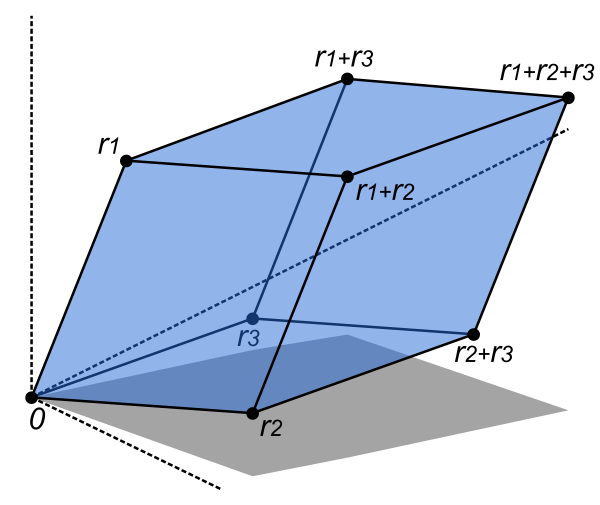
\includegraphics[width=1.5in]{600px-Determinant_parallelepiped.png}
                \end{figure}
        \end{itemize}
    \end{frame}
    \begin{frame}{$n \times n$ Matrices}
        \begin{itemize}
            \pause \item The determinant of an $n \times n$ matrix can be defined by the \textbf{Leibniz formula}.
            \pause \item A permutation of the set $\{1, 2, \cdots, n\}$ is denoted $\sigma$, and the value in the $i$-th position of the permutation $\sigma$ is denoted $\sigma_i$.
            \pause \item The set of all such permutations is denoted $S_n$.
            \pause \item For each permutation $\sigma$, $s(\sigma)$ denotes the number of inversions of $\sigma$.
            \pause \item The Leibniz formula for the determinant of an $n \times n$ matrix $A$ is $$det(A) = \sum\limits_{\sigma \in S_n} (-1) ^ {s(\sigma)} \prod\limits_{i = 1} ^ {n} a_{i, \sigma_i}$$
        \end{itemize}
    \end{frame}
    \begin{frame}{$n \times n$ Matrices}
        \begin{itemize}
            \pause \item The determinant of an $n \times n$ matrix has the following properties:
                \begin{itemize}
                    \item Swapping any pair of columns or of rows of a matrix multiplies its determinant by -1.
                    \item Multiplying a one column (row) by a scalar $k$ multiplies the value of the determinant by $k$.
                    \item Adding a multiple of one column (row) to another column (row) does not change the value of the determinant.
                \end{itemize}
        \end{itemize}
    \end{frame}
    \begin{frame}{$n \times n$ Matrices}
        \begin{itemize}
            \pause \item These properties are similar to the 3 types of the row operations.
            \pause \item Hence, we can transform a matrix into a triangular matrix by Gaussian elimination.
            \pause \item According to the definition, the determinant of a matrix in the row echelon form is the product of its entries on the main diagonal.
        \end{itemize}
    \end{frame}
    \begin{frame}{Example}
        \begin{itemize}
            \pause \item For example, the determinant of
                \begin{equation}
                    \nonumber
                    A = \left(
                    \begin{matrix}
                        -2 & 2 & 3 \\
                        -1 & 1 & 3 \\
                        2 & 0 & -1
                    \end{matrix}
                    \right)
                \end{equation}
                can be computed using the following matrices:
                \begin{equation}
                    \nonumber
                    \tiny
                    B = \left(
                    \begin{matrix}
                        -2 & 2 & 3 \\
                        0 & 0 & \frac{9}{2} \\
                        2 & 0 & -1
                    \end{matrix}
                    \right),
                    C = \left(
                    \begin{matrix}
                        -2 & 2 & 3 \\
                        0 & 0 & \frac{9}{2} \\
                        0 & 2 & -4
                    \end{matrix}
                    \right),
                    D = \left(
                    \begin{matrix}
                        -2 & 2 & 3 \\
                        0 & 2 & -4 \\
                        0 & 0 & \frac{9}{2}
                    \end{matrix}
                    \right)
                \end{equation}
        \end{itemize}
    \end{frame}
    \begin{frame}{$n \times n$ Matrices}
        \begin{itemize}
            \pause \item Here, $B$ is obtained from $A$ by adding $- \frac{1}{2}$ times the first row to the second, so $det(B) = det(A)$.
            \pause \item $C$ is obtained from $B$ by adding the first row to the third, so $det(C) = det(B)$.
            \pause \item Finally, $D$ is obtained from $C$ by exchanging the second and third rows, so $det(D) = -det(C)$.
            \pause \item The determinant of the triangular matrix $D$ is the product of its entries on the main diagonal $$det(D) = (-2) \cdot 2 \cdot \frac{9}{2} = -18$$
            \pause \item Therefore, $det(A) = -det(D) = 18$.
        \end{itemize}
    \end{frame}

    \subsection{Matrix Product}
    \begin{frame}{Matrix Product}
        \begin{itemize}
            \pause \item If $A$ is an $n \times m$ matrix and $B$ is an $m \times p$ matrix,
                \begin{equation}
                    \nonumber
                    \small
                    A = \left(
                    \begin{matrix}
                        A_{11} & A_{12} & \cdots & A_{1m} \\
                        A_{21} & A_{22} & \cdots & A_{2m} \\
                        \vdots & \vdots & \ddots & \vdots \\
                        A_{n1} & A_{n2} & \cdots & A_{nm}
                    \end{matrix}
                    \right), B = \left(
                    \begin{matrix}
                        B_{11} & B_{12} & \cdots & B_{1p} \\
                        B_{21} & B_{22} & \cdots & B_{2p} \\
                        \vdots & \vdots & \ddots & \vdots \\
                        B_{m1} & B_{m2} & \cdots & B_{mp}
                    \end{matrix}
                    \right)
                \end{equation}
                the matrix product $AB$ is defined to be an $n \times p$ matrix
                \begin{equation}
                    \nonumber
                    AB = \left(
                    \begin{matrix}
                        AB_{11} & AB_{12} & \cdots & AB_{1p} \\
                        AB_{21} & AB_{22} & \cdots & AB_{2p} \\
                        \vdots & \vdots & \ddots & \vdots \\
                        AB_{n1} & AB_{n2} & \cdots & AB_{np}
                    \end{matrix}
                    \right)
                \end{equation}
                where $(AB)_{ij} = \sum\limits_{k = 1} ^ {m} A_{ik} B_{kj}$.
        \end{itemize}
    \end{frame}
    \begin{frame}{Illustration}
        \begin{itemize}
            \pause \item
            \begin{figure}
                \centering
                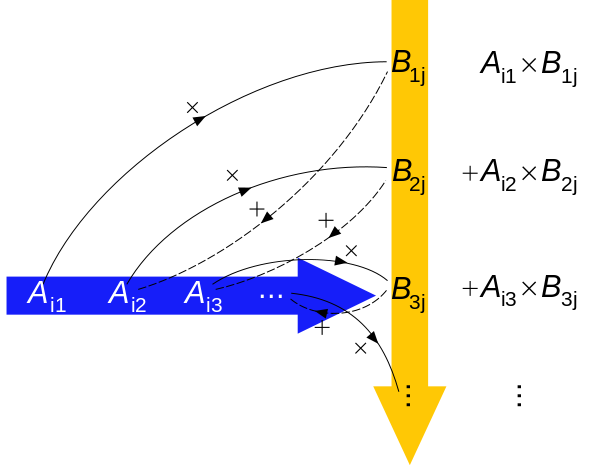
\includegraphics[width=3in]{600px-Matrix_multiplication_row_column_correspondance.png}
            \end{figure}
        \end{itemize}
    \end{frame}
    \begin{frame}{Illustration}
        \begin{itemize}
            \pause \item
            \begin{figure}
                \centering
                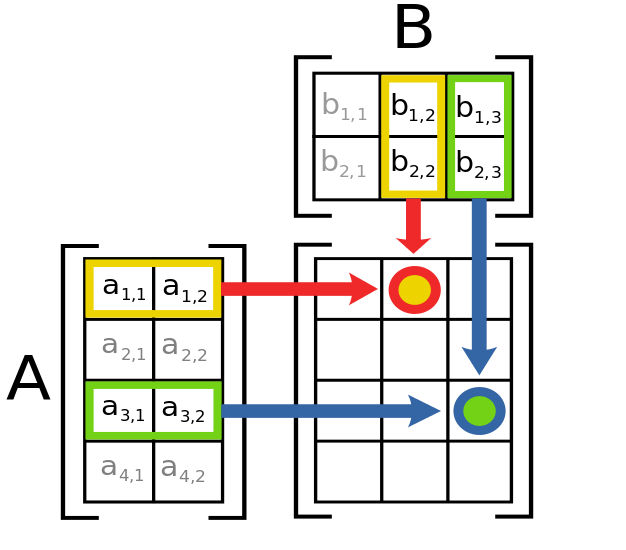
\includegraphics[width=3in]{Matrix_multiplication_diagram_2.png}
            \end{figure}
        \end{itemize}
    \end{frame}
    \begin{frame}{Properties}
        \begin{itemize}
            \pause \item \textbf{Not} commutative: $$BA \neq AB$$
            \pause \item Distributive: $$A(B + C) = AB + AC$$ $$(A + B)C = AC + BC$$
            \pause \item Scalar multiplication: $$\lambda (AB) = (\lambda A)B = A(B \lambda)$$
        \end{itemize}
    \end{frame}
    \begin{frame}{Properties}
        \begin{itemize}
            \pause \item Associative: $$ABC = (AB)C = A(BC)$$
            \pause \item Determinant: $$det\left(\prod\limits_{i = 1} ^ {n} A_i\right) = \prod\limits_{i = 1} ^ {n} det(A_i)$$
        \end{itemize}
    \end{frame}
    \begin{frame}{Powers of Matrices}
        \begin{itemize}
            \pause \item An $n \times n$ matrix $A$ is raised to a positive integer $k$ is defined as $$A ^ k = \underbrace{AA \cdots A}_{k~times}$$
            \pause \item The zero power of $A$ is defined as
                \begin{equation}
                    \nonumber
                    A ^ 0 = I_n = \left(
                    \begin{matrix}
                        1 & 0 & 0 & \cdots & 0 \\
                        0 & 1 & 0 & \cdots & 0 \\
                        0 & 0 & 1 & \cdots & 0 \\
                        \vdots & \vdots & \vdots & \ddots & \vdots \\
                        0 & 0 & 0 & \cdots & 1
                    \end{matrix}
                    \right)
                \end{equation}
        \end{itemize}
    \end{frame}
    \begin{frame}{An Optimization for Recurrence}
        \begin{itemize}
            \pause \item The powers of matrices can be used to optimize the recurrence formula.
            \pause \item A $k$-dimensional status can be expressed as a $k$-dimensional row vector
                \begin{equation}
                    \nonumber
                    \vec{x} = \left(
                    \begin{matrix}
                        x_1 & x_2 & \cdots & x_k
                    \end{matrix}
                    \right)
                \end{equation}
        \end{itemize}
    \end{frame}
    \begin{frame}{An Optimization for Recurrence}
        \begin{itemize}
            \pause \item A \textbf{companion matrix} can be expressed a $k \times k$ matrix
                \begin{equation}
                    \nonumber
                    A = \left(
                    \begin{matrix}
                        A_{11} & A_{12} & \cdots & A_{1k} \\
                        A_{21} & A_{22} & \cdots & A_{2k} \\
                        \vdots & \vdots & \ddots & \vdots \\
                        A_{k1} & A_{k2} & \cdots & A_{kk}
                    \end{matrix}
                    \right)
                \end{equation}
        \end{itemize}
    \end{frame}
    \begin{frame}{An Optimization for Recurrence}
        \begin{itemize}
            \pause \item One transformation can be expressed as
                \begin{equation}
                    \nonumber
                    \vec{x} \leftarrow \vec{x} A = \left(
                    \begin{matrix}
                        x_1 & x_2 & \cdots & x_k
                    \end{matrix}
                    \right) \left(
                    \begin{matrix}
                        A_{11} & A_{12} & \cdots & A_{1k} \\
                        A_{21} & A_{22} & \cdots & A_{2k} \\
                        \vdots & \vdots & \ddots & \vdots \\
                        A_{k1} & A_{k2} & \cdots & A_{kk}
                    \end{matrix}
                    \right)
                \end{equation}
        \end{itemize}
    \end{frame}
    \begin{frame}{An optimization for Recurrence}
        \begin{itemize}
            \pause \item Hence, $n$ transformations can be expressed as
                \begin{equation}
                    \nonumber
                    \vec{x} \leftarrow \vec{x} A = \left(
                    \begin{matrix}
                        x_1 & x_2 & \cdots & x_k
                    \end{matrix}
                    \right) \left(
                    \begin{matrix}
                        A_{11} & A_{12} & \cdots & A_{1k} \\
                        A_{21} & A_{22} & \cdots & A_{2k} \\
                        \vdots & \vdots & \ddots & \vdots \\
                        A_{k1} & A_{k2} & \cdots & A_{kk}
                    \end{matrix}
                    \right) ^ n
                \end{equation}
            \pause \item Assuming that we can compute the exponentiation of matrices $A ^ b$ in time $O\left(k ^ 3 log~b\right)$ where $A$ is a $k \times k$ matrix, the time complexity of $n$ transformations is $O\left(k ^ 3 log~n\right)$.
        \end{itemize}
    \end{frame}
    \begin{frame}{Example}
        \begin{itemize}
            \pause \item The boundary condition of the Fibonacci sequence is
                \begin{equation}
                    \nonumber
                    \begin{cases}
                        f_1 = a \\
                        f_2 = b
                    \end{cases}
                \end{equation}
                and the recurrence formula of the Fibonacci sequence is $$f_n = f_{n - 1} + f_{n - 2}$$ for $n \geq 3$.
        \end{itemize}
    \end{frame}
    \begin{frame}{Example}
        \begin{itemize}
            \pause \item Hence, the initial status is
                \begin{equation}
                    \nonumber
                    \vec{x} = \left(
                    \begin{matrix}
                        a & b
                    \end{matrix}
                    \right)
                \end{equation}
                and the companion matrix is
                \begin{equation}
                    \nonumber
                    A = \left(
                    \begin{matrix}
                        0 & 1 \\
                        1 & 1
                    \end{matrix}
                    \right)
                \end{equation}
        \end{itemize}
    \end{frame}
    \begin{frame}{Example}
        \begin{itemize}
            \pause \item Hence, to obtain the $n$-th element of the Fibonacci sequence, we transform the status for $n - 1$ times and compute
                \begin{equation}
                    \nonumber
                    \vec{x} A ^ {n - 1} = \left(
                    \begin{matrix}
                        a & b
                    \end{matrix}
                    \right) \left(
                    \begin{matrix}
                        0 & 1 \\
                        1 & 1
                    \end{matrix}
                    \right) ^ {n - 1}
                \end{equation}
            \pause \item Then, the first element of the obtained status is the $n$-th element of the Fibonacci sequence.
        \end{itemize}
    \end{frame}

	\section{Number Theory}
	\begin{frame}%[shrink]
		\frametitle{Outline}
		%\begin{multicols}{2}
			\tableofcontents[currentsection,currentsubsection]
		%\end{multicols}
	\end{frame}

    \subsection{Divisibility}
    \begin{frame}{Divisibility}
        \begin{itemize}
            \pause \item If $m > 0$ and the ratio $\frac{n}{m}$ is an integer, then we say $n$ is divided by $m$.
            \pause \item $$m | n \Leftrightarrow m > 0~and~n = mk~for~some~integer~k$$
            \pause \item If $n$ is not divided by $m$, then we say $m \nmid n$.
        \end{itemize}
    \end{frame}
    \begin{frame}{Greatest Common Divisor}
        \begin{itemize}
            \pause \item The greatest common divisor of two integers $m$ and $n$ is the greatest integer divided by both $m$ and $n$.
            \pause \item $$gcd(m, n) = max\{k: k | m~and~k | n\}$$
            \pause \item For example, $gcd(12, 18) = 6$.
            \pause \item If $n > 0$, then we have $$gcd(0, n) = n$$ since 0 is divided by any positive integer, and since n is the greatest divisor of itself.
            \pause \item $gcd(0, 0)$ is not defined.
        \end{itemize}
    \end{frame}
    \begin{frame}{Least Common Multiple}
        \begin{itemize}
            \pause \item Similarly, $$lcm(m, n) = min\{k: k > 0, m | k~and~n | k\}$$
            \pause \item If $m \leq 0$ or $n \leq 0$, then $lcm(m, n)$ is not defined.
            \pause \item Given $gcd(m, n)$, we have $$lcm(m, n) = \frac{mn}{gcd(m, n)}$$
        \end{itemize}
    \end{frame}
    \begin{frame}{Euclidean Algorithm}
        \begin{itemize}
            \pause \item The Euclidean algorithm is based on the recursive equation below:
            \pause \item $$gcd(0, n) = n$$ $$gcd(m, n) = gcd(n~mod~m, m), m > 0$$
            \pause \item For example, $gcd(12, 18) = gcd(6, 12) = gcd(0, 6) = 6$.
            \pause \item Since $n~mod~m = n - \lfloor \frac{n}{m} \rfloor m$, then any common divisor of $m$ and $n$ must be a common divisor of $m$ and $n~mod~m$.
            \pause \item The time complexity of the Euclidean algorithm is $O(log~max\{a, b\})$.
        \end{itemize}
    \end{frame}
    \begin{frame}{Extended Euclidean Algorithm}
        \begin{itemize}
            \pause \item Extended Euclidean algorithm is used to calculate $m'$ and $n'$ that satisfy the equation $$m'm + n'n = gcd(m, n)$$
            \pause \item If $m = 0$, we have $m' = 0$ and $n' = 1$.
            \pause \item Otherwise, let $r = n~mod~m$ and replace $m$ and $n$ by $r$ and $m$.
            \pause \item Then, we calculate $\overline{r}$ and $\overline{m}$ such that $$\overline{r}r + \overline{m}m = gcd(r, m)$$
        \end{itemize}
    \end{frame}
    \begin{frame}{Extended Euclidean Algorithm}
        \begin{itemize}
            \pause \item Since $r = n - \lfloor \frac{n}{m} \rfloor m$ and $gcd(r, m) = gcd(m, n)$, then we have $$\overline{r}\left(n - \lfloor \frac{n}{m} \rfloor m\right) + \overline{m}m = gcd(m, n)$$
            \pause \item Rewrite the equation, and we have $$\left(\overline{m} - \lfloor \frac{n}{m} \rfloor \overline{r}\right)m + \overline{r}n = gcd(m, n)$$
            \pause \item Hence, $m' = \overline{m} - \lfloor \frac{n}{m} \rfloor \overline{r}$ and $n' = \overline{r}$.
            \pause \item For example, $m = 12$ and $n = 18$, and we have $6 = 0 \times 0 + 1 \times 6 = 1 \times 6 + 0 \times 12 = (-1) \times 12 + 1 \times 18$.
        \end{itemize}
    \end{frame}
    \begin{frame}{Extended Euclidean Algorithm}
        \begin{itemize}
            \pause \item How to solve $ax + by = c$?
            \pause \item If $gcd(a, b) \nmid c$, then the equation has no solution.
            \pause \item Otherwise, supposing that $(x, y)$ is a pair of integers such that $ax + by = gcd(a, b)$, then $$\left(\frac{cx}{gcd(a, b)}, \frac{cy}{gcd(a, b)}\right)$$ is a pair of integers that satisfies $ax + by = c$.
        \end{itemize}
    \end{frame}
    \begin{frame}
        \begin{itemize}
            \pause \item Supposing that $(x, y)$ is a pair of integers such that $ax + by = c$, then $$\left(x + \frac{bk}{gcd(a, b)}, y - \frac{ak}{gcd(a, b)}\right), k \in \mathbb{Z}$$ is also a pair of integers that satisfies the equation.
            \pause \item The time complexity of the extended Euclidean algorithm is $O(log~max\{a, b\})$.
        \end{itemize}
    \end{frame}

    \subsection{Primes}
    \begin{frame}{Primes}
        \begin{itemize}
            \pause \item If a positive integer $p$ has exactly two factors, i.e., 1 and $p$, then $p$ is called a prime; otherwise, $p$ is a composite.
            \pause \item The first several primes are $2, 3, 5, 7, 11, 13, 17, 19, \cdots$.
            \pause \item Any positive integer $n$ can be written as a product of primes.
            \pause \item $$n = \prod\limits_{p} p^{n_p}, n_p \geq 1$$
            \pause \item Furthermore, the expansion equation above is unique.
            \pause \item This proposition is called \textbf{Fundamental Theorem of Arithmetic}.
        \end{itemize}
    \end{frame}
    \begin{frame}{Sieve of Eratosthenes}
        \begin{itemize}
            \pause \item The Sieve of Eratosthenes finds primes by iteratively marking the multiples of each prime as composites, starting with the multiples of 2.
            \pause \item (1) Create a list of consecutive integers from 2 through $n$: $(2, 3, 4, \cdots, n)$.
            \pause \item (2) Initially, let $p = 2$, the smallest prime number.
            \pause \item (3) Enumerate the multiples of $p$ by counting to $n$ from $2p$ in increments of $p$, and mark them in the list.
            \pause \item (4) Find the first number greater than $p$ in the list that is not marked. If there is no such number, stop;  otherwise, let $p$ equal this new number, and repeat from step (3).
        \end{itemize}
    \end{frame}
    \begin{frame}{Sieve of Eratosthenes}
        \begin{itemize}
            \pause \item $$T(n) = \sum\limits_{i = 1}^{n} \frac{n}{i} = n \sum\limits_{i = 1}^{n} \frac{1}{i}$$
            \pause \item According to the harmonic series, $$\sum\limits_{i = 1}^{n} \frac{1}{i} = O(log~n)$$
            \pause \item Hence, $$T(n) = n * O(log~n) = O(n~log~n)$$ i.e., the time complexity of the Sieve of Eratothenes is $O(n~log~n)$.
        \end{itemize}
    \end{frame}
    \begin{frame}{Linear Sieve}
        \begin{itemize}
            \pause \item For $i \geq 2$, denote by $\ell p(i)$ the lowest prime which divides $i$ evenly.
            \pause \item A non-prime $x$ can be written uniquely as
            \pause \item $$x = p ^ k \cdot q$$
            \pause \item where (1) $p$ is a prime, p = $\ell p(x)$;
            \pause \item ~~~~~~~~(2) $k \geq 1$;
            \pause \item ~~~~~~~~(3) $p = q$ or $p < \ell p(q)$.
        \end{itemize}
    \end{frame}
    \begin{frame}{Linear Sieve}
        \begin{itemize}
            \pause \item By the Fundamental Theorem of Arithmetic, $x$ can be written uniquely as $$x = \prod\limits_{k = 1}^{m} p_k^{n_k}$$ where $m > 1$, $p_i < p_{i + 1}$ for $1 \leq i \leq m$, \\and $m = 1$ implies $n_1 > 1$.
            \pause \item If $m = 1$, let $p = p_1$, $q = p_1$ and $k = n_1 - 1$;
            \pause \item if $m > 1$, let $p = p_1$, $q = \prod\limits_{k = 2}^{m} p_k^{n_k}$ and $k = n_1$.
            \pause \item Hence, for every integer $i$ and for every $j \leq \ell p(i)$ where $j$ is a prime, mark the product of $i$ and $j$ as a composite.
            \pause \item Since each composite $x$ is only marked by $\ell p(x)$ once, then the time complexity of the linear sieve is $O(n)$.
        \end{itemize}
    \end{frame}

    \subsection{Congruence Relation}
    \begin{frame}{Congruence Relation}
        \begin{itemize}
            \pause \item $$a \equiv b~(mod~m) \Leftrightarrow a~mod~m = b~mod~m$$
            \pause \item For example, $9 \equiv -16~(mod~5)$, since $9~mod~5 = (-16)~mod~5$.
            \pause \item Alternatively, $a \equiv b~(mod~m) \Leftrightarrow (a - b)~is~a~multiple~of~m$.
        \end{itemize}
    \end{frame}
    \begin{frame}{Congruence Relation}
        \begin{itemize}
            \pause \item If $a~mod~m = b~mod~m$, then, for some integer $k$ and $l$, we have $$a - b = (a~mod~m + km) - (b~mod~m + lm) = (k - l)m$$
            \pause \item Conversely, given that $a - b = km$, then $a = b$ when $m = 0$; otherwise, $$a~mod~m = a - \lfloor \frac{a}{m} \rfloor m$$ $$= (b + km) - \lfloor \frac{b + km}{m} \rfloor m = b - \lfloor \frac{b}{m} \rfloor m = b~mod~m$$
        \end{itemize}
    \end{frame}
    \begin{frame}{Equivalence Relation}
        \begin{itemize}
            \pause \item The congruence relation is an equivalence relation; i.e., for all $a$, $b$ and $c \in \mathbb{Z}$:
            \pause \item $a \equiv a$ (Reflexivity)
            \pause \item $a \equiv b \Rightarrow b \equiv a$ (Symmetry)
            \pause \item $a \equiv b \equiv c \Rightarrow a \equiv c$ (Transitivity)
        \end{itemize}
    \end{frame}
    \begin{frame}{Addition, Subtraction and Multiplication}
        \begin{itemize}
            \pause \item The congruence relation is compatible with addition, subtraction and multiplication on the integers.
            \pause \item If $$a \equiv b~and~c \equiv d~(mod~m)$$ then $$a \pm c \equiv b \pm d~(mod~m)$$ $$ac \equiv bd~(mod~m)$$
        \end{itemize}
    \end{frame}
    \begin{frame}{Division}
        \begin{itemize}
            \pause \item Note that the congruence relation is not compatible with division; i.e., if $ad \equiv bd$, we cannot assert that $a \equiv b$.
            \pause \item For example, $3 \times 2 \equiv 5 \times 2~(mod~4)$, but $3 \not \equiv 5$.
            \pause \item However, if $d$ and $m$ are coprime, we have $$ad \equiv bd \Leftrightarrow a \equiv b~(mod~m), a, b, d, m \in \mathbb{Z}, gcd(d, m) = 1$$
            \pause \item For example, if $m$ is not a multiple of 5, then $15 \equiv 35~(mod~m) \Rightarrow 3 \equiv 7~(mod~m)$.
        \end{itemize}
    \end{frame}
    \begin{frame}{Modular Multiplicative Inverse}
        \begin{itemize}
            \pause \item To prove this property, we are to find $d'$ and $m'$ such that $d'd + m'm = 1$.
            \pause \item Hence, if $ad \equiv bd$, then we have $add' \equiv bdd'$.
            \pause \item Since $dd' \equiv 1$, then we have $add' \equiv a$ and $bdd' \equiv b$, and therefore $a \equiv b$.
            \pause \item When considering congruence expression regarding $(mod~m)$, $d'$ serves like $\frac{1}{d}$, and hence we call it "the modular inverse of $a$ modulo $m$".
        \end{itemize}
    \end{frame}
    \begin{frame}{Division}
        \begin{itemize}
            \pause \item Furthermore, we have $$ad \equiv bd~(mod~md) \Leftrightarrow a \equiv b~(mod~m), d \neq 0$$ since $a~mod~m = b~mod~m \Leftrightarrow (a~mod~m)d = (b~mod~m)d \Leftrightarrow ad~mod~md = bd~mod~md$.
            \pause \item For example, $3 \times 2 \equiv 5 \times 2~(mod~4) \Rightarrow 3 \equiv 5~(mod~2)$.
        \end{itemize}
    \end{frame}
    \begin{frame}{Division}
        \begin{itemize}
            \pause \item More generally, we have $$ad \equiv bd~(mod~m) \Leftrightarrow a \equiv b~\left(mod~\frac{m}{gcd(d, m)}\right)$$ where $a, b, d, m \in \mathbb{Z}$.
            \pause \item We can multiply $ad \equiv bd$ by $d'$ where $d'd + m'm = gcd(d, m)$, which gives $$a \cdot gcd(d, m) \equiv b \cdot gcd(d, m)~(mod~m)$$ and divide it by $gcd(d, m)$.
        \end{itemize}
    \end{frame}
    \begin{frame}{Module}
        \begin{itemize}
            \pause \item Moreover, we have $$a \equiv b~(mod~md) \Rightarrow a \equiv b~(mod~m), d \in \mathbb{Z}$$ since any multiple of $md$ must be a multiple of $m$.
            \pause \item Conversely, $$a \equiv b~(mod~m)~and~a \equiv b~(mod~n) \Leftrightarrow a \equiv b~(mod~lcm(m, n))$$ where $m, n \in \mathbb{Z}, m, n > 0$, \\since if $a - b$ is a common multiple of $m$ and $n$, then it must be a multiple of $lcm(m, n)$.
            \pause \item For example, if we know that $a \equiv b~(mod~12)$ and $a \equiv b~(mod~18)$, then we have $a \equiv b~(mod~36)$.
        \end{itemize}
    \end{frame}
    \begin{frame}{Module}
        \begin{itemize}
            \pause \item The module $m$ can be decomposed into factors that are pairwise coprime.
            \pause \item If $m = \prod\limits_{p} p^{m_p}$, then we have $$a \equiv b~(mod~m) \Leftrightarrow a \equiv b~\left(mod~p^{m_p}\right)$$ for each $p$.
        \end{itemize}
    \end{frame}

    \subsection{Chinese Remainder Theorem}
    \begin{frame}{Chinese Remainder Theorem}
        \begin{itemize}
            \pause \item Let $m_1, m_2, \cdots, m_k$ be integers greater than 1, and $M = \prod\limits_{i = 1}^{k} m_i$.
            \pause \item The Chinese remainder theorem asserts that if the $m_i$ are pairwise coprime, and if $a_1, a_2, \cdots a_k$ are any integers, then there exist integers $x$ such that
                \begin{equation}
                    \nonumber
                    \begin{cases}
                        x \equiv a_1~(mod~m_1) \\
                        x \equiv a_2~(mod~m_2) \\
                        \quad \cdots \\
                        x \equiv a_k~(mod~m_k)
                    \end{cases}
                \end{equation}
            and any two such $x$ are congruent modulo $M$; i.e., there is exactly one such $x$ in the range $0 \leq x < M$.
        \end{itemize}
    \end{frame}
    \begin{frame}{Solution}
        \begin{itemize}
            \pause \item Let $M_i = \frac{M}{m_i}$ and $t_i = M_i^{-1}~(mod~m_i)$.
            \pause \item Since $M_i = \frac{M}{m_i} = \frac{m_1 m_2 \cdots m_k}{m_i}$, we have $$M_i \equiv 0~(mod~m_j), i \neq j$$
            \pause \item Since $t_i = M_i^{-1}~(mod~m_i)$ and since $M_i$ and $m_i$ are coprime, we have $$a_i t_i M_i \equiv a_i~(mod~m_i)$$
        \end{itemize}
    \end{frame}
    \begin{frame}{Solution}
        \begin{itemize}
            \pause \item Let $X \equiv \sum\limits_{i = 1}^{k} a_i t_i M_i~(mod~M)$.
            \pause \item Since $m_i | M$, we have $$X \equiv \sum\limits_{i = 1}^{k} a_i t_i M_i \equiv a_i~(mod~m_i)$$ for each $i$ such that $1 \leq i \leq k$.
            \pause \item Hence, $X$ is a solution to the system of congruent equations above.
        \end{itemize}
    \end{frame}
    \begin{frame}{Non-Coprime Chinese Remainder Theorem: Method 1}
        \begin{itemize}
            \pause \item What if the $m_i$ are not coprime?
            \pause \item Consider 2 equations:
                \begin{equation}
                    \nonumber
                    \begin{cases}
                        x \equiv a_1~(mod~m_1) \\
                        x \equiv a_2~(mod~m_2)
                    \end{cases}
                \end{equation}
            \pause \item Considering combining the 2 equations, we have $$a_1 + m_1 x_1 = a_2 + m_2 x_2$$
            \pause \item Rearranging gives $$m_1 x_1 - m_2 x_2 = a_2 - a_1$$
        \end{itemize}
    \end{frame}
    \begin{frame}{Non-Coprime Chinese Remainder Theorem: Method 1}
        \begin{itemize}
            \pause \item That $gcd(m_1, m_2) \nmid (a_2 - a_1)$ indicates that the system of congruent equations has no solution.
            \pause \item Otherwise, the extended Euclidean algorithm gives the minimal positive value of $x_1$ and hence $x = a_1 + m_1 x_1$.
            \pause \item The result of combining the 2 equations is $$x~mod~lcm(m_1, m_2)$$
            \pause \item Combine 2 equations at a time, and eventually we obtain the solution to the system of congruent equations.
        \end{itemize}
    \end{frame}
    \begin{frame}{Non-Coprime Chinese Remainder Theorem: Method 2}
        \begin{itemize}
            \pause \item For each prime factor $p | M$, find the maximum power of $p$ in all the $m_i$, and set a new system of congruent equations using the maximum power of each $p$ as moduli:
                \begin{equation}
                    \nonumber
                    \begin{cases}
                        x \equiv a_1'~(mod~p_1^{n_1}) \\
                        x \equiv a_2'~(mod~p_2^{n_2}) \\
                        \quad \cdots \\
                        x \equiv a_{k'}'~(mod~p_{k'}^{n_{k'}})
                    \end{cases}
                \end{equation}
        \end{itemize}
    \end{frame}
    \begin{frame}{Non-Coprime Chinese Remainder Theorem: Method 2}
        \begin{itemize}
            \pause \item Use the Chinese remainder theorem to solve the new system of congruent equations.
            \pause \item Since we only consider the maximum power of each prime factor $p$, a check on the validity of the answer over the original system of congruent equations is required.
        \end{itemize}
    \end{frame}

    \subsection{Euler's Totient Function}
    \begin{frame}{Euler's Totient Function}
        \begin{itemize}
            \pause \item Euler's Totient Function, or Euler's Phi Function, written as $\varphi(n)$, counts the positive integers up to $n$ that are relatively prime to $n$; i.e., it is defined as the number of integer $k$ in the range $1 \leq k \leq n$ for which $gcd(n, k) = 1$.
            \pause \item For example, $\varphi(9) = 6$, since the 6 numbers 1, 2, 4, 5, 7 and 8 are all relatively prime to 9, but the other 3 numbers in the range, 3, 6 and 9, are not, because $gcd(9, 3) = gcd(9, 6) = 3$ and $gcd(9, 9) = 9$.
        \end{itemize}
    \end{frame}
    \begin{frame}{Multiplicative Function}
        \begin{itemize}
            \pause \item Euler's Totient Function is a multiplicative function, meaning that if $m$ and $n$ are relatively prime, then $$\varphi(mn) = \varphi(m) \varphi(n)$$
            \pause \item For example, $\varphi(12) = \varphi(3) \varphi(4) = 2 \times 2 = 4$.
            \pause \item Since $\varphi(n)$ is multiplicative, it can be computed along with the linear sieve.
        \end{itemize}
    \end{frame}
    \begin{frame}{Euler's Totient Function}
        \begin{itemize}
            \pause \item If $p$ is a prime and $k \geq 1$, then $$\varphi(p ^ k) = p ^ k - p ^ {k - 1} = p ^ {k - 1} (p - 1) = p ^ k \left(1 - \frac{1}{p} \right)$$
            \pause \item Since $p$ is a prime, the only possible values of $gcd(p ^ k, m)$ are $1, p, p ^ 2, \cdots, p ^ k$, and the only way for $gcd(p ^ k, m)$ to not equal 1 is for $m$ to be a multiple of $p$, i.e., $p, 2p, 3p, \cdots, p ^ {k - 1} p = p ^ k$.
            \pause \item Hence, the other $\left(p ^ k - p ^ {k - 1}\right)$ numbers are all relatively prime to $p ^ k$.
        \end{itemize}
    \end{frame}
    \begin{frame}{Euler's Product Formula}
        \begin{itemize}
            \pause \item The fundamental theorem of arithmetic states that if $n > 1$, there is a unique expression of $n$, $$n = \prod\limits_{k = 1}^{m} p_k^{n_k}$$ where $p_1 < p_2 < \cdots < p_m$ are prime numbers and each $n_i \geq 1$.
            \pause \item The multiplicative property gives $$\varphi(n) = \varphi\left(p_1^{n_1}\right) \varphi\left(p_2^{n_2}\right) \cdots \varphi\left(p_m^{n_m}\right)$$
        \end{itemize}
    \end{frame}
    \begin{frame}{Euler's Product Formula}
        \begin{itemize}
            \pause \item The formula for $\varphi(p ^ k)$ gives $$\varphi(n) = p_1^{n_1}\left(1 - \frac{1}{p_1}\right) p_2^{n_2}\left(1 - \frac{1}{p_2}\right) \cdots p_m^{n_m}\left(1 - \frac{1}{p_m}\right)$$
            \pause \item Rearranging gives $$\varphi(n) = p_1^{n_1} p_2^{n_2} \cdots p_m^{n_m} \left(1 - \frac{1}{p_1}\right) \left(1 - \frac{1}{p_2}\right) \cdots \left(1 - \frac{1}{p_m}\right)$$
            \pause \item That is, $$\varphi(n) = n \prod\limits_{k = 1}^{m} \left(1 - \frac{1}{p_k}\right)$$
        \end{itemize}
    \end{frame}
    \begin{frame}{Euler's Product Formula}
        \begin{itemize}
            \pause \item For example, $\varphi(36) = \varphi(2 ^ 2 3 ^ 2) = 36 \left(1 - \frac{1}{2}\right) \left(1 - \frac{1}{3}\right) = 36 \cdot \frac{1}{2} \cdot \frac{2}{3} = 12$.
            \pause \item Indeed, there are 12 positive integers coprime with 36 and lower than 36: 1, 5, 7, 11, 13, 17, 19, 23, 25, 29, 31, 35.
        \end{itemize}
    \end{frame}
    \begin{frame}{Euler's Theorem}
        \begin{itemize}
            \pause \item If $a$ and $n$ are relatively prime, then $$a ^ {\varphi(n)} \equiv 1~(mod~n)$$
            \pause \item The special case where $n$ is prime is known as \textbf{Fermat's Little Theorem}: $$a ^ p \equiv a~(mod~p), p~is~prime$$
        \end{itemize}
    \end{frame}

    \subsection{Modular Multiplicative Inverse}
    \begin{frame}{Modular Multiplicative Inverse}
        \begin{itemize}
            \pause \item In modular arithmetic, the modular multiplicative inverse of an integer $a$ modulo $m$ is an integer $x$ such that $$ax \equiv 1~(mod~m)$$
            \pause \item The modular multiplicative inverse of $a$ modulo $m$ exists iff. $a$ and $m$ are coprime, i.e., iff. $gcd(a, m) = 1$.
            \pause \item If the modular multiplicative inverse of $a$ modulo $m$ exists, the operation of division by $a$ modulo $m$ can be defined as multiplying by the inverse of $a$, i.e., $a ^ {-1}$.
        \end{itemize}
    \end{frame}
    \begin{frame}{Example}
        \begin{itemize}
            \pause \item Suppose we wish to find the modular multiplicative inverse of 3 modulo 11.
            \pause \item $$x \equiv 3 ^ {-1}~(mod~11)$$
            \pause \item This is the same as find $x$ such that $$3x \equiv 1~(mod~11)$$
            \pause \item Working in $\mathbb{Z}_{11}$ we find that $3 \cdot 4 = 12 \equiv 1~(mod~11)$, and there are no other values of $x$ in $\mathbb{Z}_{11}$ that also satisfy the congruence.
            \pause \item Hence, the modular multiplicative inverse of 3 modulo 11 is 4.
        \end{itemize}
    \end{frame}
    \begin{frame}{Extended Euclidean Algorithm}
        \begin{itemize}
            \pause \item The modular multiplicative inverse is the solution to $$ax \equiv 1~(mod~m)$$
            \pause \item That is, $$ax - 1 = qm$$
            \pause \item $$ax - qm = 1$$
            \pause \item This is the exact form that the extended Euclidean algorithm solves, assuming that $gcd(a, m) = 1$.
            \pause \item The algorithm runs in time $O(log~m)$.
        \end{itemize}
    \end{frame}
    \begin{frame}{Euler's Theorem}
        \begin{itemize}
            \pause \item According to Euler's theorem, if $a$ is coprime to $m$, i.e., gcd(a, m) = 1, then $$a ^ {\varphi(m)} \equiv 1~(mod~m)$$ where $\varphi(m)$ is Euler's totient function.
            \pause \item Hence, the modular multiplicative inverse can be found directly: $$a ^ {\varphi(m) - 1} \equiv a ^ {-1}~(mod~m)$$
        \end{itemize}
    \end{frame}
    \begin{frame}{Euler's Theorem}
        \begin{itemize}
            \pause \item When $m$ is a prime, the modular inverse is given by $$a ^ {-1} \equiv a ^ {m - 2}~(mod~m)$$
            \pause \item Assuming that the value $\varphi(m)$ is known and that we can compute the exponentiation $a ^ b$ in time $O(log~b)$, the time complexity of calculating the modular inverse is $O(log~m)$.
        \end{itemize}
    \end{frame}
    \begin{frame}{Inverse of Factorials}
        \begin{itemize}
            \pause \item According to the definition of the modular multiplicative inverse, we have $$(n!) ^ {-1} \equiv \frac{1}{n!} \equiv \frac{n + 1}{(n + 1)!}$$
            \pause \item Hence, given $((n + 1)!) ^ {-1}$, we can compute $(n!) ^ {-1}$ by $$(n!) ^ {-1} \equiv (n + 1)((n + 1)) ^ {-1}$$
            \pause \item Therefore, we can compute $(i!) ^ {-1}$ for each $i$ in the range $0 \leq i \leq n$ in time $O(n)$.
        \end{itemize}
    \end{frame}
    \begin{frame}{Inverse of 1 through $n$}
        \begin{itemize}
            \pause \item Suppose that $a = \lfloor \frac{y}{x} \rfloor$ and $b = y~mod~x$ where $y$ is prime and $1 < x < y$.
            \pause \item Hence, we have $$ax + b \equiv 0~(mod~y)$$
            \pause \item Multiply the equation by $x ^ {-1} b ^ {-1}$, and we have $$ab ^ {-1} + x ^ {-1} \equiv 0~(mod~y)$$ and hence $$x ^ {-1} \equiv -ab ^ {-1}~(mod~y)$$
        \end{itemize}
    \end{frame}
    \begin{frame}{Inverse of 1 through $n$}
        \begin{itemize}
            \pause \item Replace $a$ and $b$ by $\lfloor \frac{y}{x} \rfloor$ and $y~mod~x$ respectively, and we have $$x ^ {-1} \equiv - \lfloor \frac{y}{x} \rfloor \cdot (y~mod~x) ^ {-1}~(mod~y)$$
            \pause \item Given $1 ^ {-1}$ through $(x - 1) ^ {-1}$, we can compute $x ^ {-1}$ in time $O(1)$.
            \pause \item Therefore, we can compute $1 ^ {-1}$ through $n ^ {-1}$ in time $O(n)$.
        \end{itemize}
    \end{frame}

    \section{Numerical Analysis}
    \begin{frame}%[shrink]
		\frametitle{Outline}
		%\begin{multicols}{2}
			\tableofcontents[currentsection,currentsubsection]
		%\end{multicols}
	\end{frame}

    \subsection{Lagrange Interpolation}
    \begin{frame}{Polynomial Interpolation}
        \begin{itemize}
            \pause \item Given a set of $n + 1$ data points $\left(x_i, y_i\right)$, where no two $x_i$ are the same, the polynomial interpolation problem is to find a polynomial $p$ of degree at most $n$ such that $$p(x_i) = y_i, i = 0, 1, \cdots, n$$
            \pause \item It can be proved that such a polynomial $p$ exists and is unique.
        \end{itemize}
    \end{frame}
    \begin{frame}{Lagrange Interpolation}
        \begin{itemize}
            \pause \item The \textbf{interpolation polynomial in the Lagrange form} is a linear combination $$L(x) = \sum\limits_{j = 0}^{n} y_j l_j(x)$$
            \pause \item The \textbf{Lagrange basis polynomials} are
            \begin{equation}
                \nonumber
                \begin{aligned}
                    l_j(x) &= \prod\limits_{0 \leq m \leq n \atop m \neq j} \frac{x - x_m}{x_j - x_m} \\
                    &= \frac{\left(x - x_0\right)}{\left(x_j - x_0\right)} \cdots \frac{\left(x - x_{j - 1}\right)}{\left(x_j - x_{j - 1}\right)} \frac{\left(x - x_{j + 1}\right)}{\left(x_j - x_{j + 1}\right)} \cdots \frac{\left(x - x_n\right)}{\left(x_j - x_n\right)}
                \end{aligned}
            \end{equation}
            where $0 \leq j \leq n$.
        \end{itemize}
    \end{frame}
    \begin{frame}{Lagrange Interpolation}
        \begin{itemize}
            \pause \item For all $i \neq j$, $l_j(x)$ includes the term $\left(x - x_i\right)$ in the numerator, so the whole product will be 0 at $x = x_i$:
            \begin{equation}
                \nonumber
                \begin{aligned}
                    l_{j \neq i}\left(x_i\right) &= \prod\limits_{m \neq j} \frac{x_i - x_m}{x_j - x_m} \\
                    &= \frac{\left(x_i - x_0\right)}{\left(x_j - x_0\right)} \cdots \frac{\left(x_i - x_i\right)}{\left(x_j - x_i\right)} \cdots \frac{\left(x_i - x_n\right)}{\left(x_j - x_n\right)} = 0
                \end{aligned}
            \end{equation}
            \pause \item On the other hand, $$l_i\left(x_i\right) = \prod\limits_{m \neq i} \frac{x_i - x_m}{x_i - x_m} = 1$$
        \end{itemize}
    \end{frame}
    \begin{frame}{Lagrange Interpolation}
        \begin{itemize}
            \pause \item It follows that
            \begin{equation}
                \nonumber
                \begin{cases}
                    y_i l_i\left(x_i\right) = y_i \\
                    y_j l_j\left(x_i\right) = 0, j \neq i
                \end{cases}
            \end{equation}
            \pause \item Hence, at each point $x_i$, $$L\left(x_i\right) = y_i + 0 + 0 + \cdots + 0 = y_i$$ showing that $L$ interpolates the function exactly.
        \end{itemize}
    \end{frame}
    \begin{frame}{Example 1}
        \begin{itemize}
            \pause \item We wish to interpolate $f(x) = x ^ 2$ over the range $1 \leq x \leq 3$, given these three points:
            \begin{equation}
                \nonumber
                \begin{aligned}
                    x_0 = 1 \quad f(x_0) = 1 \\
                    x_1 = 2 \quad f(x_1) = 4 \\
                    x_2 = 3 \quad f(x_2) = 9
                \end{aligned}
            \end{equation}
            \pause \item The interpolating polynomial is
            \small{
            \begin{equation}
                \nonumber
                \begin{aligned}
                    L(x) &= 1 \cdot \frac{x - 2}{1 - 2} \cdot \frac{x - 3}{1 - 3} + 4 \cdot \frac{x - 1}{2 - 1} \cdot \frac{x - 3}{2 - 3} + 9 \cdot \frac{x - 1}{3 - 1} \cdot \frac{x - 2}{3 - 2} \\
                    &= x ^ 2
                \end{aligned}
            \end{equation}}
        \end{itemize}
    \end{frame}
    \begin{frame}{Example 2}
        \begin{itemize}
            \pause \item We wish to interpolate $f(x) = x ^ 3$ over the range $1 \leq x \leq 3$, given these three points:
            \begin{equation}
                \nonumber
                \begin{aligned}
                    x_0 = 1 \quad f(x_0) = 1 \\
                    x_1 = 2 \quad f(x_1) = 8 \\
                    x_2 = 3 \quad f(x_2) = 27
                \end{aligned}
            \end{equation}
            \pause \item The interpolating polynomial is
            \small{
            \begin{equation}
                \nonumber
                \begin{aligned}
                    L(x) &= 1 \cdot \frac{x - 2}{1 - 2} \cdot \frac{x - 3}{1 - 3} + 8 \cdot \frac{x - 1}{2 - 1} \cdot \frac{x - 3}{2 - 3} + 27 \cdot \frac{x - 1}{3 - 1} \cdot \frac{x - 2}{3 - 2} \\
                    &= 6 x ^ 2 - 11 x + 6
                \end{aligned}
            \end{equation}}
        \end{itemize}
    \end{frame}
    \begin{frame}{Time Complexity and a Special Case}
        \begin{itemize}
            \pause \item The Lagrange Interpolation runs in time $O(n ^ 2)$.
            \pause \item Given that the polynomial interpolation problem is computed in the residue system modulo $p$, where $p$ is prime, and that $x_i = i$, the original Lagrange polynomial $$L(x) = \sum\limits_{j = 0}^{n} y_j l_j(x) = \sum\limits_{j = 0}^{n} y_j \prod\limits_{m \neq j} \frac{x - x_m}{x_j - x_m}$$ can be converted to $$L(x) = \sum\limits_{j = 0}^{n} y_j \prod\limits_{m \neq j} \frac{x - m}{j - m}$$
        \end{itemize}
    \end{frame}
    \begin{frame}{Time Complexity and a Special Case}
        \begin{itemize}
            \pause \item Rewrite the expression above, and we have $$L(x) = \sum\limits_{j = 0}^{n} y_j \frac{\prod\limits_{i = x - k}^{x - j - 1} i \prod\limits_{i = x - j + 1}^{x} i}{(-1) ^ {n - j}j!(n - j)!}$$
            \pause \item Assuming that we have preprocessed prefix products, suffix products, factorials and modular multiplicative inverses, the Lagrange interpolation can run in time $O(n)$.
        \end{itemize}
    \end{frame}

    %\section{Combinatorial Mathematics}
    %\begin{frame}%[shrink]
	%	\frametitle{Outline}
	%	%\begin{multicols}{2}
	%		\tableofcontents[currentsection,currentsubsection]
	%	%\end{multicols}
	%\end{frame}

    \section{}
    \begin{frame}
        \centering
        \huge Thank you!
    \end{frame}

\end{CJK}
\end{document}
